
\chapter{Měření parametrů}
\label{chap:param}

\begin{wrapfigure}{r}{0.5\textwidth}
    \vspace*{0.75cm}
    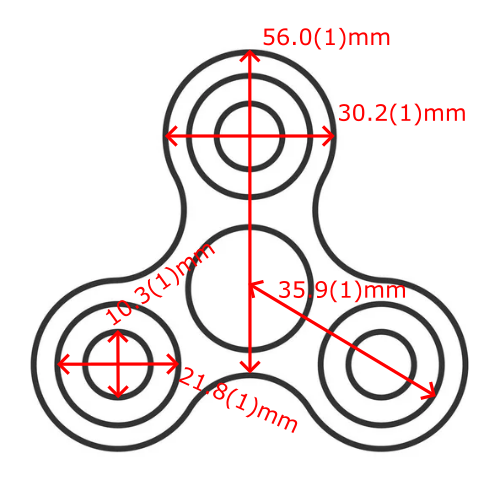
\includegraphics[width=0.45\textwidth]{dims.png}
    \centering
    \caption{Ilustrace spinneru společně s vyznačenými rozměry}
    \label{fig:spinner_size}
\end{wrapfigure}

\section{Rozměry spinneru}
\label{sec:spinner_size}
K popsání spinneru nejdříve určíme jeho rozměry (viz \autoref{fig:spinner_size}).
Nejdůležitější rozměr pro nás bude vzdálenost osy otáčení od místa, kde budou umístěny magnety.
To je v našem případě $r = 35.9(1)mm$.

Vzhledem k tomu, že na sebe spinnery mohou vzájemně působit pouze magnetickými silami, jak je řečeno v zadání, není třeba řešit zbytek geometrie spinneru v budoucích modelech.
Spinner budeme dále modelovat pouze jako $n$ magnetických dipólů, které se otáčejí kolem středu $S$ a pevně si udržují své relativní pozice.
Tomuto celkovému systému definujeme moment setrvačnosti podle následujícího měření.
\section{Moment setrvačnosti}
\label{sec:moment_of_inertia}
{\raggedright
    K určení momentu setrvačnosti spinneru bylo využito idealizace spinneru jakožto fyzického kyvadla, pro které platí: \cite{physical_pendulum}
}
\begin{equation}
    \label{eq:mag_pend}
    \omega = \sqrt{\frac{mgr}{I}}
\end{equation}
A po vyjádření z rovnice \ref{eq:mag_pend} získáváme:
\begin{equation}
    \label{eq:mom_inert}
    I = \frac{mgr}{\omega^2} = \frac{mgr}{4\pi^2f^2}
\end{equation}
Nyní stačí změřit frekvenci kmitů zavěšeného spinneru s několika magnety na jednom z jeho ramen a dopočítat moment setrvačnosti.

\begin{wrapfigure}{r}{0.5\textwidth}
    \vspace*{-0.75cm}
    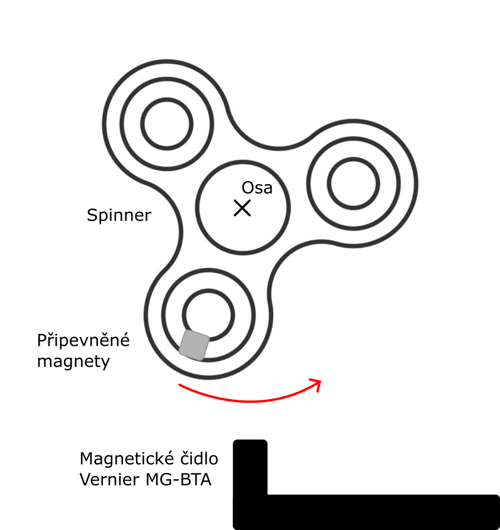
\includegraphics[width=0.45\textwidth]{mom_inert_setup.png}
    \centering
    \caption{Ilustrace aparatury pro měření frekvence kmitů spinneru}
    \label{fig:spinner_pendulum_aparature}
\end{wrapfigure}
\subsection{Aparatura}
Po připevnění šesti neodymových magnetů o jednotkové hmotnosti $0.92(1) g$ byl spinner připevněn pevně ve své ose otáčení.
Pod takto zavěšený spinner bylo umístěno magnetické čidlo Vernier MG-BTA, které zaznamenávalo, jak blízko se magnety nacházejí.
Po umístění spinneru mimo rovnovážnou polohu byl ponechán oscilovat a záznam průběhu magnetického pole v čase byl čidlem nasnímán (viz \autoref{fig:spinner_pendulum_recording}).
\vspace{40pt}

{\raggedright
    \subsection{Analýza měření a výsledky}
    Průběh následně analyzujeme pomocí programovacího jazyku \texttt{Python} \cite{python} a knihovny \texttt{scipy} \cite{scipy}.
    Námi kýžená maxima, která odpovídají půlperiodě kmitu, vyhledáme použitím funkce \texttt{scipy.signal.find\_peaks} a z jejich počtu jsme schopni určit počet period, kterými kyvadlo prošlo za určený čas.
}

\begin{wrapfigure}{r}{1\textwidth}
    \includegraphics[width=1\textwidth]{spin_pendulum_field_rec.png}
    \centering
    \caption[Nasnímaný průběh magnetické indukce v čase pro spinnerové kyvadlo]{Nasnímaný průběh magnetické indukce v čase (modře) pro spinnerové kyvadlo. Peaky, označující uplynutí jedné půlperiody, jsou vyznačeny červeně.}
    \label{fig:spinner_pendulum_recording}
\end{wrapfigure}

\clearpage

Máme-li tedy pole\footnote{$|p|$ označuje počet prvků pole $p$; $p_{min}$ označuje čas prvního peaku; $p_{max}$ označuje čas posledního peaku.} $p$ všech časů nalezených peaků, je výpočet frekvence následující:
\begin{equation}
    \label{eq:freq_from_peaks}
    f = \frac{ |p| - 1}{2(p_{max} - p_{min})} = 1.00(1)Hz
\end{equation}

Dosazením do předchozí rovnice \ref{eq:mom_inert} získáváme výslednou hodnotu\footnote{Tato hodnota je srovnatelná s jinými zdroji dostupnými online (viz. \cite{spinner_mom_inert_external}).}:
\begin{equation}
    \label{eq:mom_inert_results}
    I = 4.80(50) \cdot 10^{-5} kg \cdot m^2
\end{equation}

\subsection{Popis skriptu}

V níže připnutém ústřižku kódu \ref{code:1} nejdříve načteme použité knihovny:
\texttt{numpy} \cite{numpy} pro provedení konvoluce,
\texttt{matplotlib} pro vytvoření grafu \ref{fig:spinner_pendulum_recording} \cite{matplotlib} a nakonec
\texttt{scipy}, kde využijeme funkce \texttt{find\_peaks}, jak již bylo zmíněno.

Prvním krokem je načtení dat ze souboru \texttt{kyvadlo.csv} a jejich převedení z textového formátu do 2D pole pojmenovaného \texttt{data}.
Dále izolujeme data jednotlivých os do separátních proměnných \texttt{xdata}, \texttt{ydata}.

\texttt{ydata} vyhladíme, abychom se zbavili šumu, a to pomocí konvoluce použitím funkce \texttt{numpy.convolve}.
Délku 1D konvoluční matice jsme zvolili $m = 15$ a konvoluční matice délky $m$ by v našem případě obecně vypadala takto:

\begin{equation}
    \label{eq:conv_matrix_avg}
    M_{conv} =
    \underbrace{
        \begin{pmatrix}
            \frac{1}{m} & \frac{1}{m} & ... & \frac{1}{m}
        \end{pmatrix}
    }_{m\text{ krát}}
\end{equation}

Tato konvoluční matice provádí aritmetický průměr $m$ za sebou jdoucích hodnot.

Nyní provedeme hledání peaků na vyhlazených datech pomocí funkce \texttt{find\_peaks}, která akceptuje další dobrovolné argumenty:
\begin{enumerate}[topsep=0pt, partopsep=0pt]
    \setlength{\itemsep}{0pt}%
    \setlength{\parskip}{0pt}%
    \item height: určuje minimální absolutní velikost peaku
    \item threshold: minimální rozdíl dvou sousedních hodnot, aby bod mohl být peakem
    \item distance: minimální indexová vzdálenost dvou peaků
\end{enumerate}

Poté určíme časový interval, kde se peaky nacházejí (a přidáme na každou stranu 0.5 sekundy pro přehlednost grafu),
a vygrafujeme původní naměřená data (modře) společně s pozicemi peaků (červeně). Dále označíme osy.

Nakonec dopočítáme frekvenci kmitů kyvadla podle vzorce \ref{eq:freq_from_peaks} a vypíšeme ji.

\clearpage

\lstinputlisting[language=Python, caption=Kód k analyzování spinnerového kyvadla, label=code:1]{./prilohy/snippets/c1.py}

\section{Remanence $\vec{B}_r$}
\label{sec:remanence_measurement}

K určení remanence našich magnetů využijeme dvou různých metod. Jedna z nich bude založena na silové interakci magnetů a jedna na magnetem vytvořeném poli.

\subsection{Určení remanence přes magnetické pole}

Prvním způsobem, jak určit hodnotu remanentní magnetizace našich magnetů, je měření magnetického pole pomocí magnetometru mobilního telefonu.
Aplikace \texttt{Phyphox} umožňuje čtení těchto dat, která následně analyzujeme.

Měření provedeme pro sloupce 2 a 3 magnetů, abychom ověřili, zda je náš způsob měření konzistentní.
Dále také měříme větší neodymový magnet, jehož parametry nám nejsou známé, a který budeme používat v některých budoucích experimentech.
Abychom odstranili pozadí tvořené magnetickým polem země, provedeme měření magnetického pole magnetu v jedné orientaci a poté magnet otočíme a změříme hodnotu při opačné orientaci.
K získání výsledku jednoduše odečteme rozdíl naměřených hodnot, což bude dvojnásobek velikosti magnetického pole tvořeného magnetem.
Je zřejmé, že tímto odstraníme z měření jiné, neměnné, zdroje magnetických polí.

Kromě provádění měření pro různé počty a velikosti magnetů, budeme také měřit pole v různých vzdálenostech od magnetu, abychom dále potvrdili, zda jsou měření a náš model konzistentní.
Celkem provedeme tedy měření 2 magnetů, 3 magnetů a velkého magnetu pro vzdálenosti 5 cm, 10 cm, 20 cm a 30 cm.

\subsubsection{Analýza měření}
Výstupem aplikace \texttt{Phyphox} jsou sobory typu \texttt{.csv}, neboli \textit{"Comma separated values"} \cite{csv}.
Toto je poměrně čitelný a přívětivý formát ukládání dat, který v \texttt{Pythonovém} skriptu načteme pomocí funkce \texttt{open} (stejně jako v kódu \ref{code:1}).
V kódu budeme používat tyto knihovny:
\texttt{numpy},
\texttt{matplotlib} pro vytvoření grafu \ref{fig:mag_field_recording_2mag_10cm},
\texttt{scipy}, kde využijeme funkci \texttt{curve\_fit}, a konečně knihovnu
\texttt{math} \cite{pymath}.
Poté ručně určíme názvy všech datových souborů a časové intervaly, na kterých jsou magnety orientovány k snímači a od snímače.

Po načtení dat vyjmeme pouze hodnoty ve dříve zmíněných intervalech a najdeme jejich průměrnou hodnotu a odchylky.
Z rozdílu průměrných hodnot magnetického pole při obou otočeních magnetů určíme velikost magnetického pole generovaného pouze magnetem (očištěného od pozadí).
Z odchylek také určíme celkovou odchylku výsledné hodnoty.

Následně pro každé měření vytvoříme graf (příkladem je \autoref{fig:mag_field_recording_2mag_10cm}).

\lstinputlisting[language=Python, caption=Kód k určení průměrné hodnoty magnetického pole a odchylek, label=code:2]{./prilohy/snippets/c2.py}

\begin{wrapfigure}{c}{1\textwidth}
    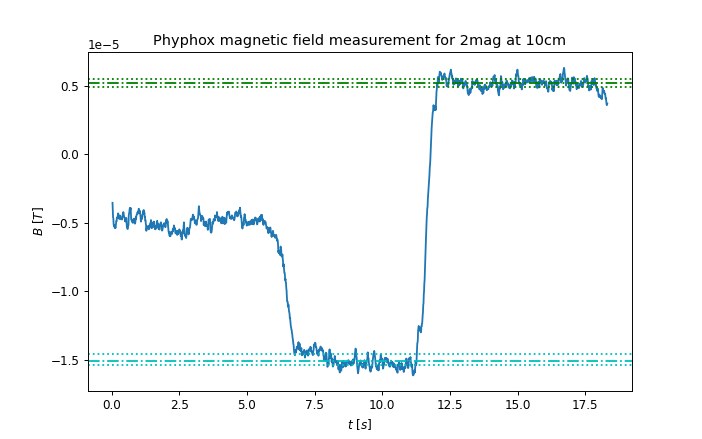
\includegraphics[width=1\textwidth]{mag_field_measurement_2mag_10cm.png}
    \centering
    \caption[Nasnímaný průběh magnetické indukce v čase pro účely měření remanence]{Nasnímaný průběh magnetické indukce v čase (modře) pro určení remanence. Průměrné hodnoty horní orientace (zeleně čerchovaně) a dolní orientace (modře čerchovaně). Odpovídající odchylky jsou znázorněny tečkovaně. Výsledná hodnota magnetické indukce tohoto příkladu, tedy dvou magnetů ve vzdálenosti 10 cm, je: $B = 1.01(8) \cdot 10^{-5} T$}
    \label{fig:mag_field_recording_2mag_10cm}
\end{wrapfigure}

\clearpage

\begin{wrapfigure}{r}{0.5\textwidth}
    \vspace*{0.5cm}
    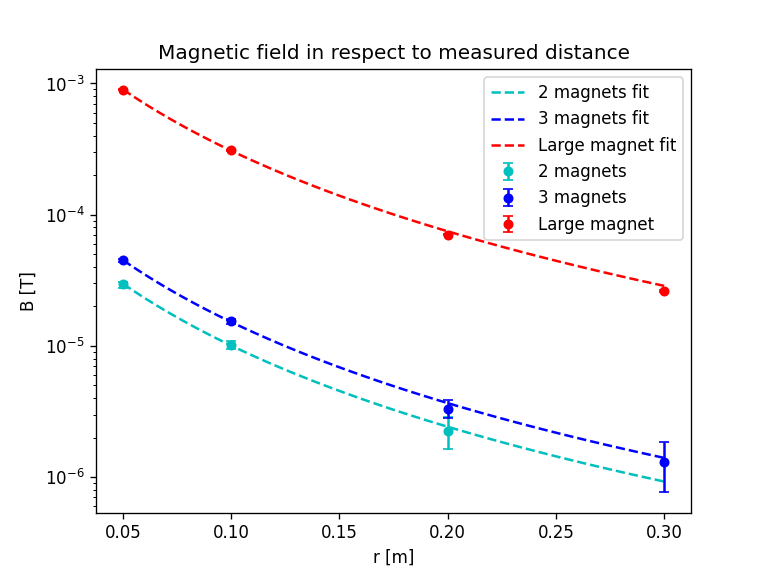
\includegraphics[width=0.45\textwidth]{B_field_in_distance.png}
    \centering
    \caption[Závislost magnetické indukce na vzdálenosti]{Závislost magnetické indukce na vzdálenosti. Sledujeme, že $B \propto r^{-3}$}
    \label{fig:B_in_dist}
\end{wrapfigure}

Po zanalyzování všech měření můžeme vytvořit graf závislosti $B$ na vzdálenosti (viz \autoref{fig:B_in_dist}).
Pro určení $B_r$ z naměřených hodnot zjednodušíme vzorec \ref{eq:B} tak, že nahradíme vektory pouze jejich velikostmi, čímž získáme následující vzorec:

\begin{equation}
    \label{eq:B_reduced}
    |B| = \frac{{\mu}_0 |m|}{2\pi r^3}
\end{equation}

Zde si všimněme úměrnosti $B \propto r^{-3}$, kterou také sledujeme v našich naměřených datech.
Následným dosazením rovnice \ref{eq:mag_mom_remanence} a vyjádřením remanence získáváme:

\begin{equation}
    \label{eq:Br_from_B}
    |B_r| = \frac{2\pi r^3 |B|}{V}
\end{equation}

Pro každou naměřenou hodnotu $B$ následně dopočítáme odpovídající $B_r$ a výsledky později (společně s výsledky druhého měření) zobrazíme v souhrnném grafu \ref{fig:rem_final}.

\subsection{Určení remanence přes sílu}

Druhý způsob, kterým jsme schopni určit remanenci, je skrze přitahování (resp. odpuzování) jednoho magnetu k (resp. od) druhému magnetu. Posazením jednoho magnetu na váhu a sledováním změny měřené hmotnosti jsme z gravitačního zrychlení schopni dopočítat působící sílu druhého magnetu, který je umístěn v určité výšce. Zároveň první magnet podložíme lehkou, tlustou a nemagnetickou vrstvou (např. blokem polystyrenu), abychom zabránili interakci magnetu s kovovými částmi váhy.

\begin{wrapfigure}{r}{0.5\textwidth}
    \vspace*{-1cm}
    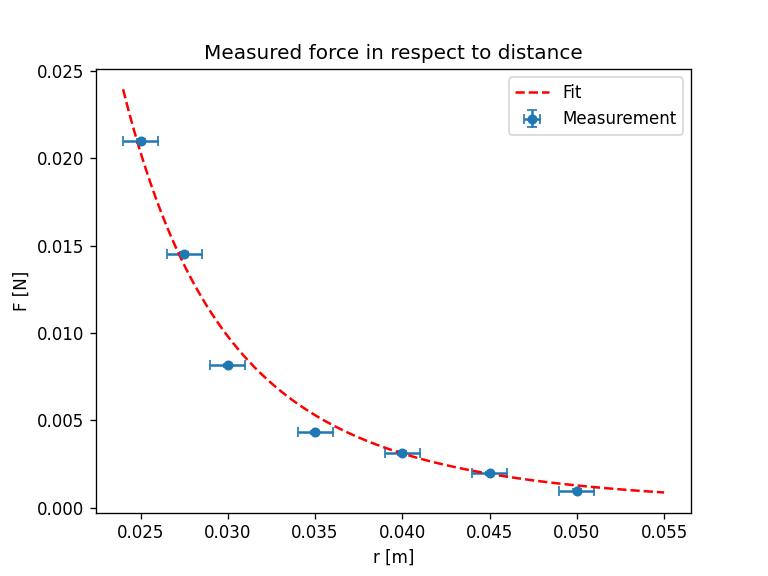
\includegraphics[width=0.45\textwidth]{F_in_distance.png}
    \centering
    \caption[Závislost magnetické síly na vzdálenosti]{Závislost magnetické síly na vzdálenosti. Sledujeme, že $F \propto r^{-4}$}
    \label{fig:mag_force_in_dist}
\end{wrapfigure}

Výhodou této metody je, že jsme schopni přesněji měřit slabší magnety, jelikož je můžeme dát blíže. V předchozí kapitole jsme nebyli schopni přiblížit magnety dostatečně blízko ke snímači telefonu kvůli rozměrům telefonu samotného.
Toto měření provádíme pouze pro 1 magnet, jelikož nám pro něj chybí výsledky z měření pomocí magnetického pole (ze dříve zmíněných důvodů). Výsledky můžeme vidět na grafu \ref{fig:mag_force_in_dist}.

\clearpage

Výpočet remanence provedeme podobně jako u rovnice \ref{eq:B_reduced}, a to náhradou vektorů za jejich velikosti v rovnici \ref{eq:F_m}. Tím jsme ji schopni zjednodušit na následující podobu:

\begin{equation}
    \label{eq:F_reduced}
    |F| =  \frac{3 {\mu}_0}{2\pi r^4}|m|^2
\end{equation}

Po dosazení rovnice \ref{eq:mag_mom_remanence} a vyjádření remanence získáváme:

\begin{equation}
    \label{eq:Br_from_F}
    B_r = \sqrt{\frac{2\pi {\mu}_0 r^4 F}{3 V^2}}
\end{equation}

Výsledné hodnoty $B_r$ zobrazíme v jednotném grafu \ref{fig:rem_final} v následující kapitole.

\subsection{Výsledky}

Výsledky obou způsobů měření sjednotíme do grafu závislosti $B_r$ na vzdálenosti (viz \autoref{fig:rem_final}).
Očekáváme, že se $B_r$ v závislosti na vzdálenosti nebude měnit, a pro každé měření určíme souhrnnou hodnotu pomocí optimalizace fitu konstantní funkcí. Výsledkem všech měření bude aritmetický průměr těchto souhrnných hodnot.

\begin{wrapfigure}{r}{0.5\textwidth}
    \vspace*{-0.5cm}
    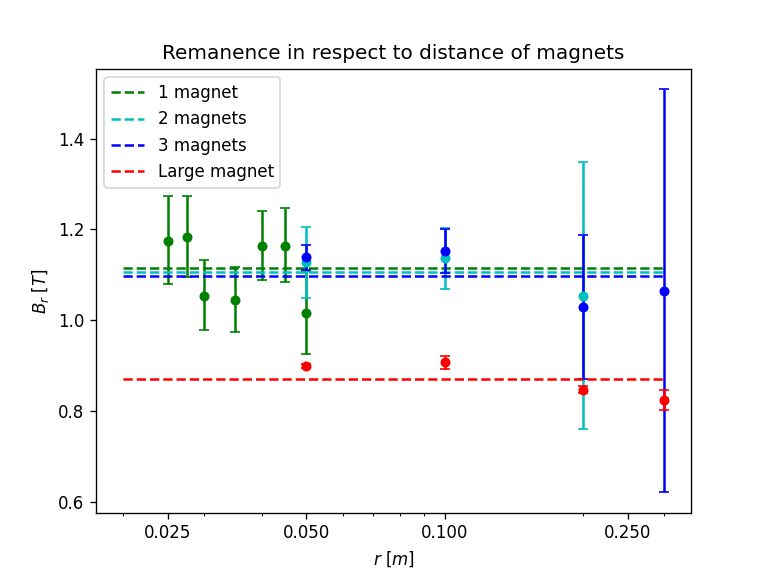
\includegraphics[width=0.5\textwidth]{Final_remanence.png}
    \centering
    \caption[Souhrnný graf všech měření remanence]{Souhrnný graf všech měření remanence. Ve výpočtu výsledné hodnoty $B_r$ není započítávána remanence velkého magnetu, jelikož není součástí stejné várky magnetů a budeme s ním nakládat později jinak.}
    \label{fig:rem_final}
\end{wrapfigure}

Výsledná hodnota remanence našich krychlových magnetů je\footnote{Námi naměřené hodnoty jsou srovnatelné s externími zdroji (viz. \cite{magnet_grades}).}:
$$
    B_r = 1.10(13) T
$$

a našeho velkého magnetu je:
$$
    B_{r_{xl}} = 0.87(5)T
$$

Prvním důvodem, proč je remanence většího magnetu znatelně nižší, může být jeho stáří. Dalším důvodem může být skutečnost, že takto velký magnet náš model není schopen popsat jako jediný magnetický dipól.

\clearpage
